\documentclass[12pt]{article}
\usepackage[a4paper, total={6in, 9in}]{geometry}
\usepackage{verbatim}
\usepackage[dvips]{epsfig}
\usepackage{fp}
\usepackage{color}
%\usepackage[decimalsymbol=comma]{siunitx}
%\sisetup{round-mode=places,round-precision=4}
\usepackage{pgf}
\usepackage{url}
\usepackage[colorlinks=true]{hyperref}
\usepackage{longtable}
\usepackage{eurosym}
\usepackage{enumitem}

\begin{document}

\section*{Abstract}

Extension of simulator functionality may result in the unintentional creation of a monolithic software platform. This greatly increases the difficulty of extending simulator software code to support new functionality such as efficient multi-scale modelling. Analysis suggests that the difficulties of simulator extensibility faced by many software developers originates in a primary focus on the biological and mathematical implementation of a model, at the expense of considering the underlying software architecture. This limits software development efforts, thus simulator functionality, and ultimately simulator extensibility. Here, axioms defining the domain of computational neuroscience that have been extracted from twenty years of global use and experience in GENESIS, are presented. They provide a logical framework that organizes the approach to multi-scale simulation that is here presented. A framework underpins the modular design of the CBI federated software architecture employed to reconfigure the GENESIS simulator. This has resolved many problems associated with multi-scale modelling that previously existed with this simulator. The approach to development of simulator structure and function is outlined by describing essential components of a simulator for multi-scale modelling. Careful consideration of the issues identified greatly facilitates the development of a simulator capable of transparently supporting multi-scale biological modelling across levels ranging from the ionic and molecular to complete systems.

\begin{figure}[h!t]
  \begin{center}
    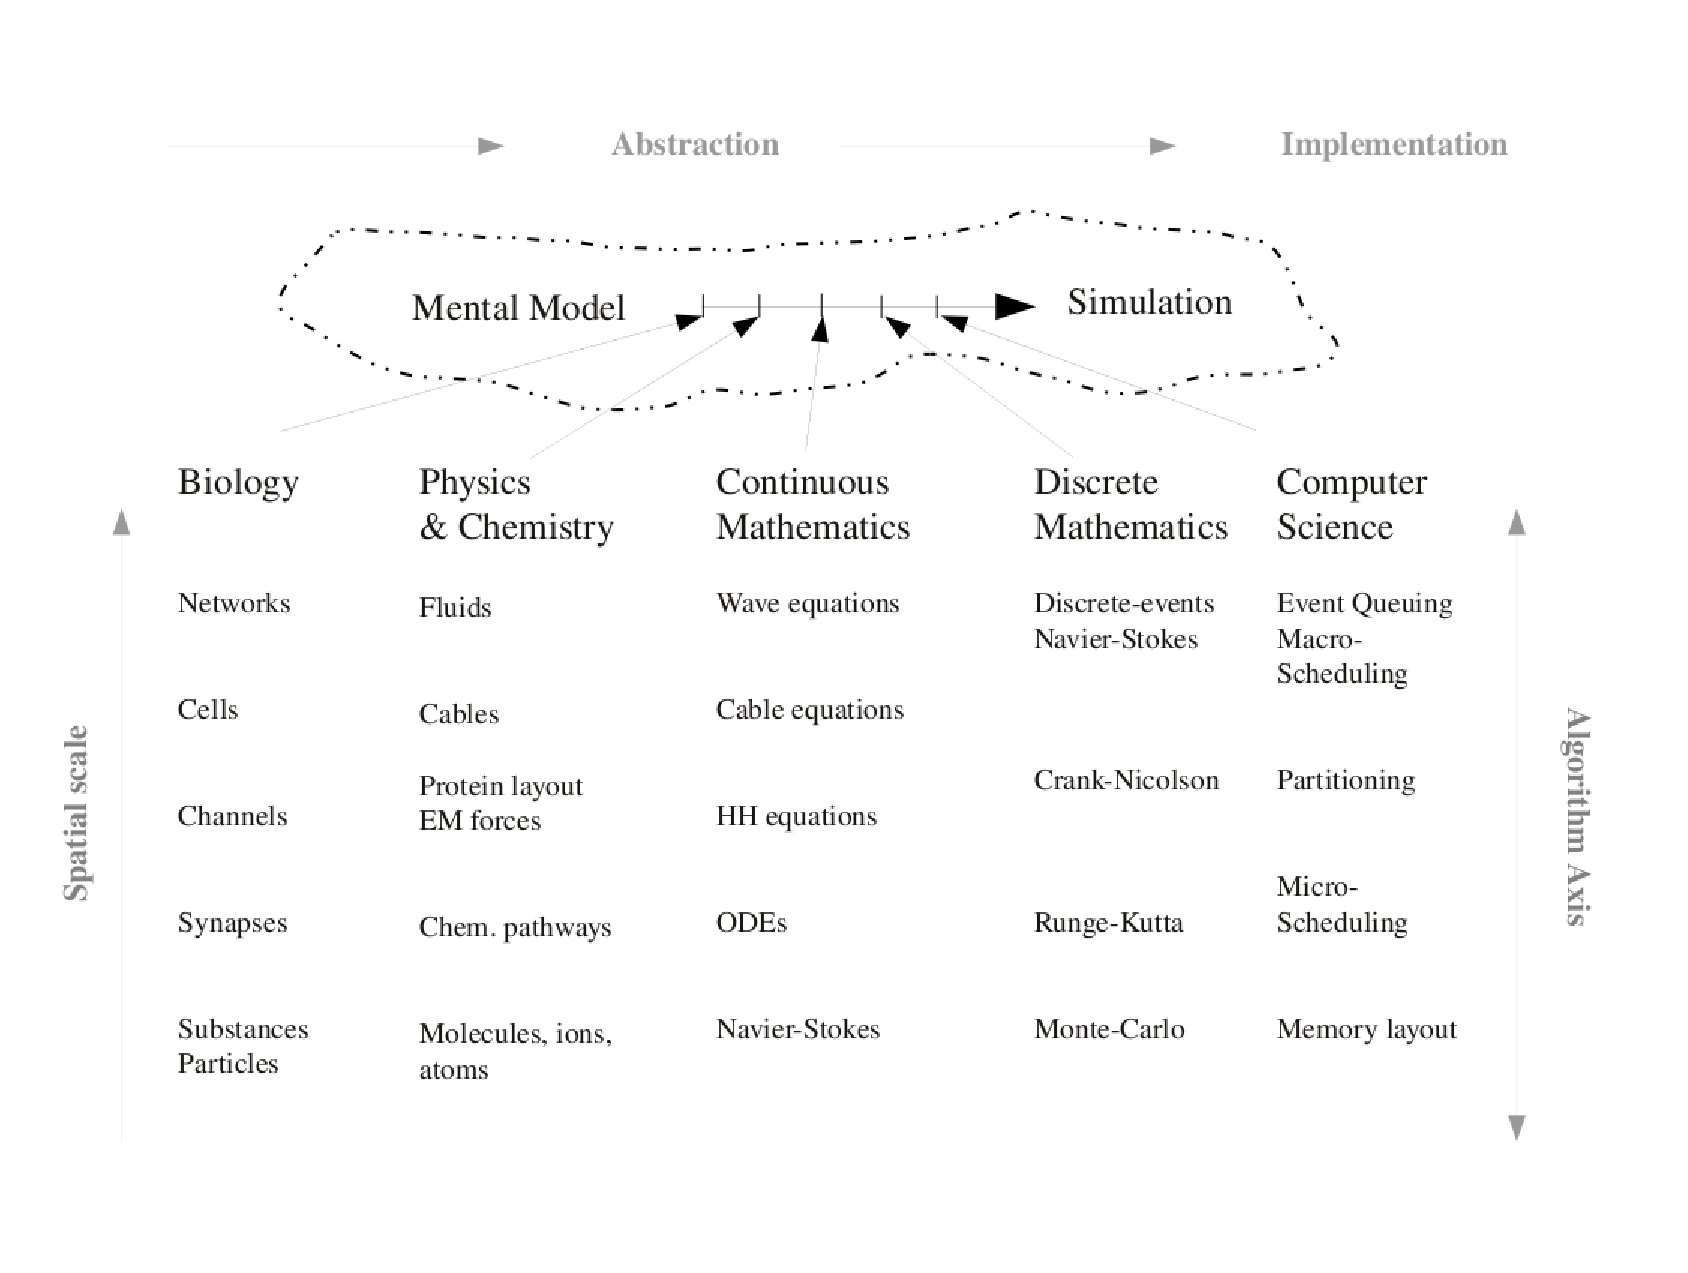
\includegraphics[width=4in]{figures/NS-abstraction-implementation.eps}
  \end{center}
  \caption{ {\bf A Multi-Scale Path from Mental Model to Simulation.} }
  \label{fig:mental-model-simulation-path}
\end{figure}

\end{document}
